
%(BEGIN_QUESTION)
% Copyright 2013, Tony R. Kuphaldt, released under the Creative Commons Attribution License (v 1.0)
% This means you may do almost anything with this work of mine, so long as you give me proper credit

Examine this process trend showing the PV, SP, and Output of a loop controller:

$$\includegraphics[width=15.5cm]{i02634x01.eps}$$

Based on what you see here, determine the following:

\begin{itemize}
\item{} Whether this is an open-loop or a closed-loop response
\item{} Whether the controller is (or needs to be) {\it direct-acting} or {\it reverse-acting}
\item{} If possible, identify any problems with the field instrumentation
\item{} If possible, identify any problems with the controller PID tuning
\item{} Qualitatively identify the kind of PID tuning we will need for robust control
\end{itemize}



\underbar{file i02634}
%(END_QUESTION)





%(BEGIN_ANSWER)

This is a {\it closed-loop test}, based on the fact the output signal responds dynamically to the changing process variable, as well as to the step-change in setpoint.

\vskip 10pt

This is a {\it reverse-acting} controller: the output steps up when the setpoint steps up (implying the output would step down if the process variable stepped up).

\vskip 10pt

This process does exhibit some dead time as well as lag time, which explains the setpoint overshoot.  A field check of the control element (valve) might be good to do, so see that it is not sticking and causing dead time. 

\vskip 10pt
  
The controller tuning actually looks pretty good here.  The only problem is the slight overshoot of setpoint, which may or may not be significant depending on the specific process and the needs of operations personnel.  If this overshoot is deemed excessive, we might wish to turn down the proportional action (gain), based on the fact the PV and output waves seem to hit their respective peaks at nearly the same time (characteristic of proportional-dominant action).

\vskip 10pt

Given the existence of dead time and lag time together, we must be careful not to use too much proportional action lest the loop oscillate.  Derivative action could be very useful in taming the effects of lag time.

%(END_ANSWER)





%(BEGIN_NOTES)


%INDEX% Process troubleshooting: diagnosing problem via trend recording

%(END_NOTES)


